
\chapter{语言模型实验及实验结果分析}
在前面两章中,本文按照章节分别介绍本文中使用的方法具体过程。在本章中,本文将会展示并行层次概率计算算法的实验结果,并且在第二小节中展现实验结果,以及与其他加速算法的对比。
\section{实验数据集}
\begin{table}
  \centering
  \caption{WikiText-2, WikiText-103 和 One Billion Words 数据集统计指标。 Number of tokens for train, valid and test, vocabulary size, and fraction of out-of-vocabulary (OOV) rate.\label{tab:dataset}}
\begin{tabular}{llrrrrr}
\toprule
数据集& 类型& 文章数 & 句子数量 &  单词数量 &词表大小 & OOV (\%) \\ \midrule
\multirow{3}{*}{Wikitext-2} &训练集& 600 & 36,718 & 2,088,628 & \multirow{3}{*}{33,278} & \multirow{3}{*}{2.6\%} \\
&验证集& 60 &3,760 & 217,646  & &\\
&测试集& 60 & 4,358 & 245,569 & &\\
\midrule
\multirow{3}{*}{Wikitext-103} &训练集& 28,475 &  1,801,350 &  103,227,021 & \multirow{3}{*}{267,735} & \multirow{3}{*}{0.4\%} \\
&验证集& 60 &3,760 & 217,646  & &\\
&测试集& 60 & 4,358 & 245,569 & &\\
\midrule
\multirow{3}{*}{One Billion Word} &训练集& --- &30,301,028&768,646,526&   \multirow{3}{*}{793,471} &   \multirow{3}{*}{0.28\%} \\
 &验证集& --- &  6,075 &   153,583 &&\\
 &测试集 & --- &  6,206 &   159,354 &&\\
\bottomrule
\end{tabular}
\end{table}
\section{评价指标}
\begin{equation}\label{equ:ppl}
   \mathrm{PPL}(w_1,\cdots,w_T)=\sqrt[T]{\frac{1}{\prod_{t=1}^T p(w_t|w_{1:t-1})}}
\end{equation}

\begin{equation}\label{equ:wer}
  \mathrm{WER} = \frac{\text{插入单词数 + 删除单词数 + 替换单词数}}{\text{全部单词数量}}
\end{equation}

\section{实验分析}
\begin{figure}
%\setlength{\abovecaptionskip}{0pt}
%\setlength{\belowcaptionskip}{0pt}
  \centering
  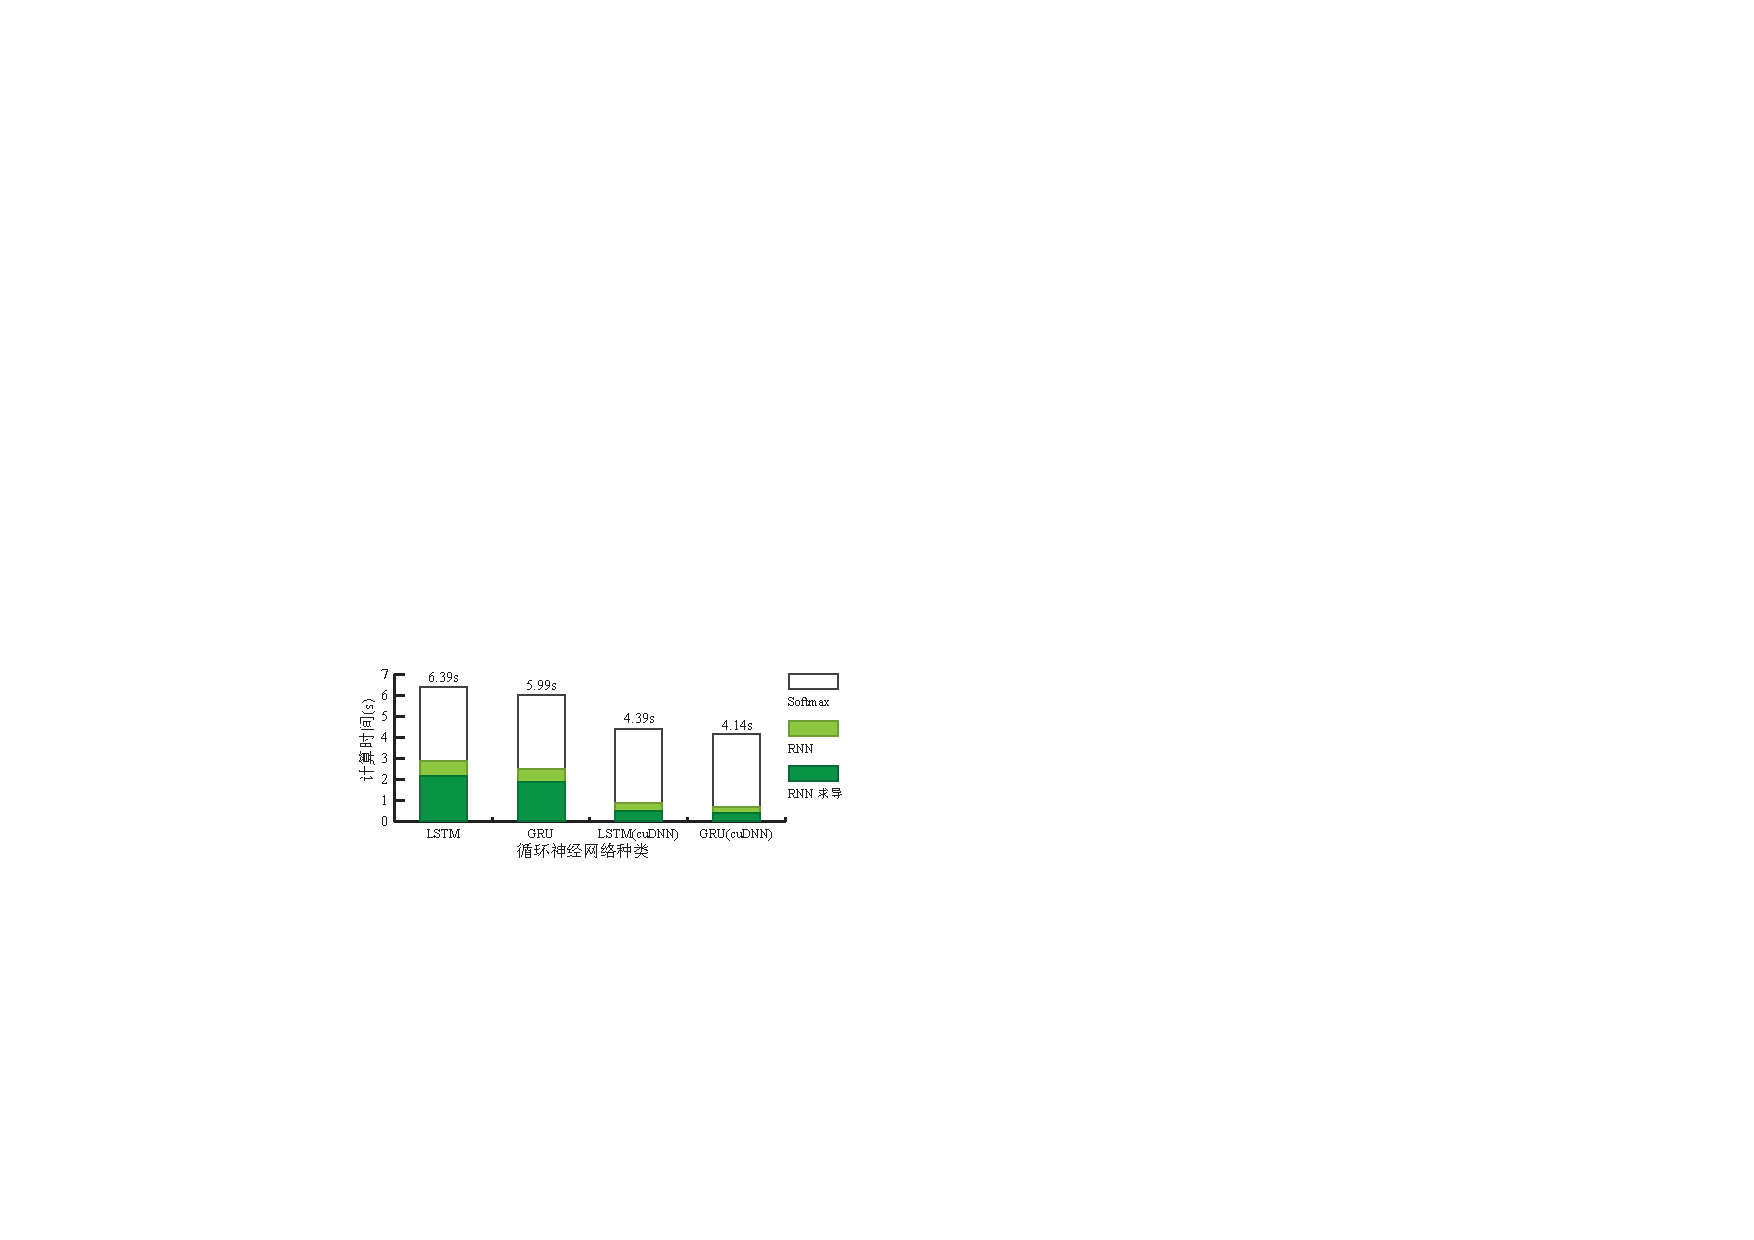
\includegraphics[width=0.6\columnwidth]{./figures/rnn_timing.pdf}
  \caption{Calculation Time of three modules with different recurrent cells on the Wikitext-103 dataset.}\label{fig:rnn_timing}
\end{figure}
\begin{figure}
%\setlength{\abovecaptionskip}{0pt}
%\setlength{\belowcaptionskip}{0pt}
  \centering
  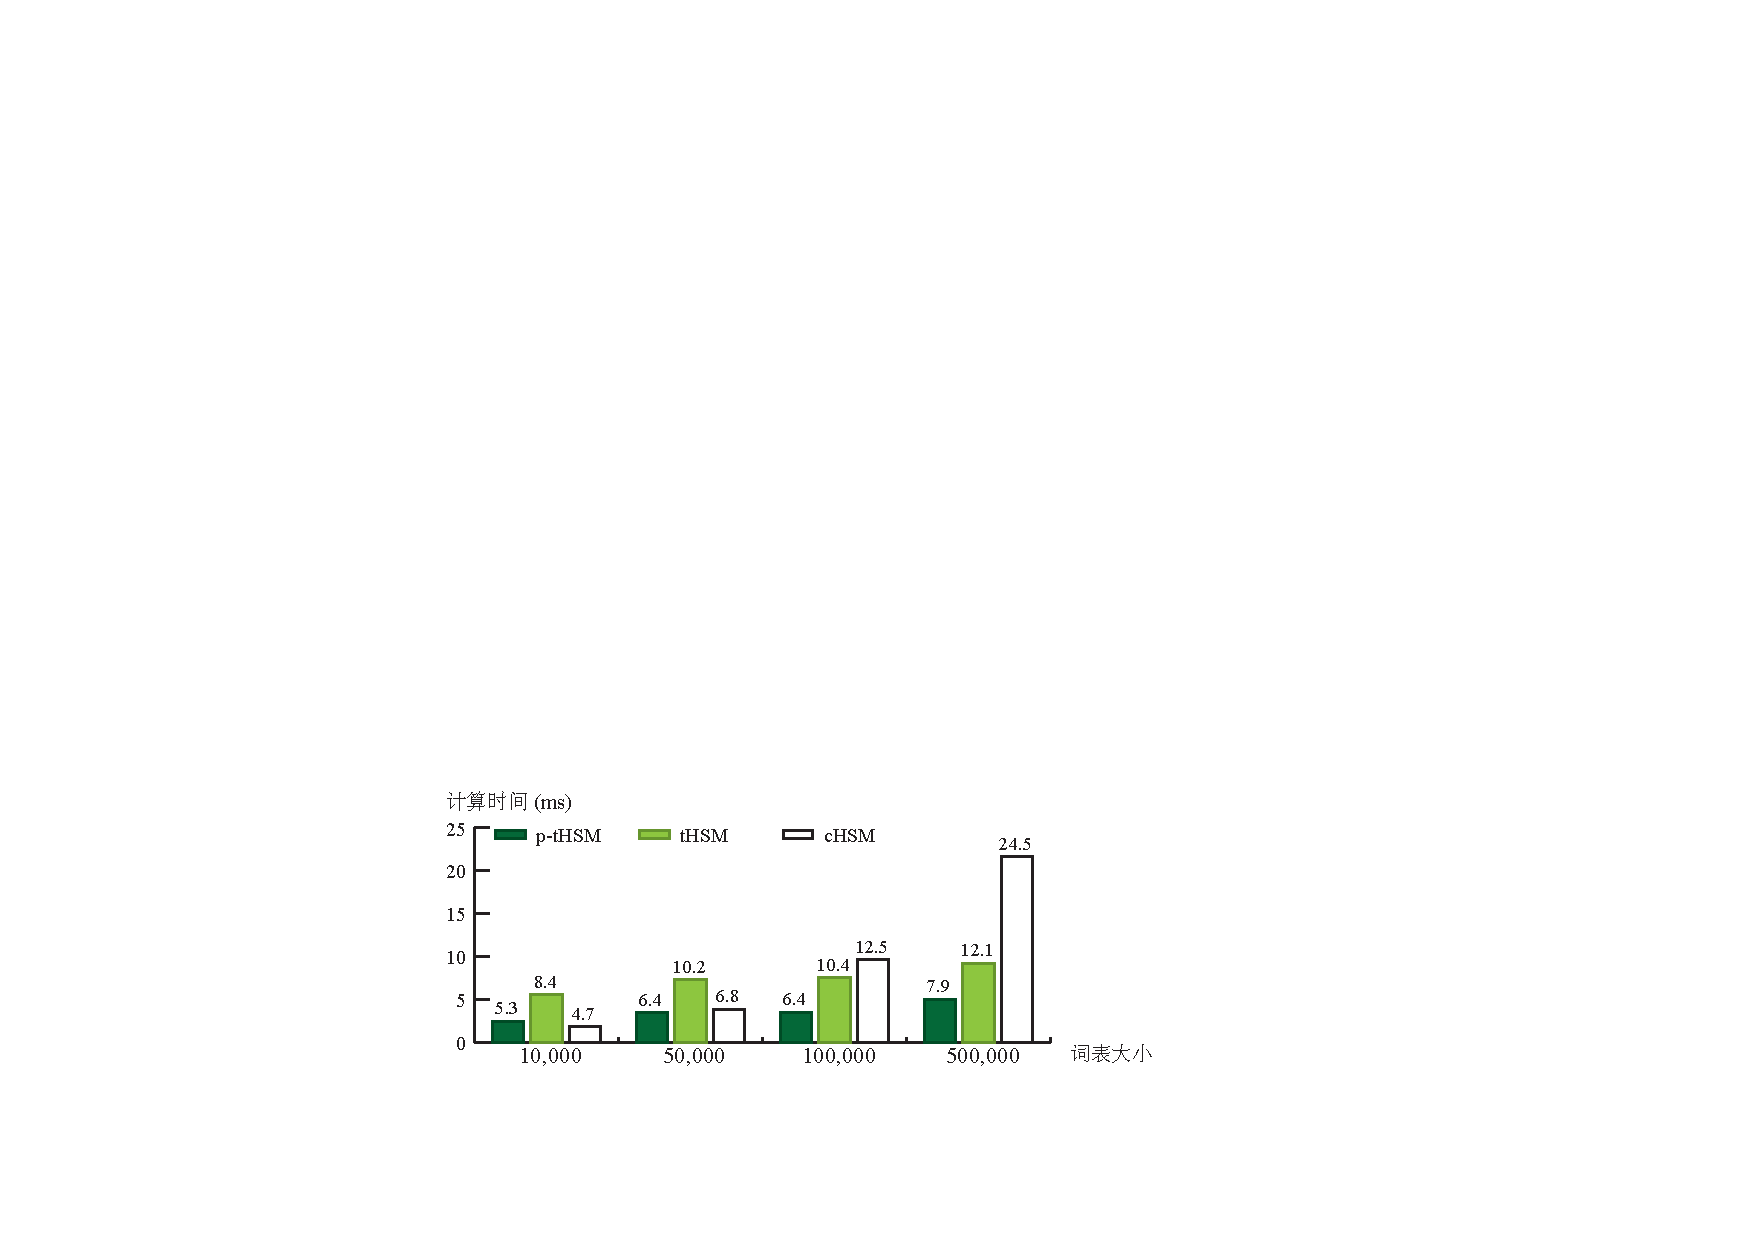
\includegraphics[width=0.6\columnwidth]{./figures/all_time.pdf}
  \caption{Scalability of cHSM, tHSM and p-tHSM algorithms with relevance to the vocabulary size.}\label{fig:hsm_benchmark}
\end{figure}
\begin{table}[!t]
%\setlength{\abovecaptionskip}{0pt}
%\setlength{\abovedisplayskip}{0pt}
  \centering
  \caption{Runtime time and memory comparison on GPUs and CPUs with WikiText-103 Dataset.\label{tab:time}}
\begin{tabular}{lccccc}
  \toprule
 \multirow{2}{*}{Methods}  &\multirow{2}{*}{Runtime Memory} &\multicolumn{2}{c}{Total Time (ms)} & \multicolumn{2}{c}{Forward Time (ms)}   \\
   \cmidrule(lr){3-4}  \cmidrule(lr){5-6}
	& & CPU&GPU & CPU& GPU \\ \midrule
Softmax & $\mathcal{|HV|}$ &510.4  &262.1&352.2& 62.9 \\
cHSM    & $2\mathcal{|H|\sqrt{|V|}}$&506.5  &\textbf{40.6}&28.7&14.6 \\
tHSM    &$\mathcal{|H|}$&1,004.0 &444.4 & 8.1&  5.6   \\
p-tHSM  &$\mathcal{|H|\log{|V|}}$ &\textbf{383.5}&	86.4 &\textbf{7.0}&	\textbf{1.4} \\
  \bottomrule
\end{tabular}
\end{table}


\begin{table}[t]
%\setlength{\abovecaptionskip}{0pt}
%\setlength{\abovedisplayskip}{0pt}
  \centering
  \caption{在Wikitext-2数据集上,cHSM 算法采用不同聚类算法的PPL 和 WER 结果 .\label{table:clustering}}
  \begin{tabular}{lclccc} \toprule
聚类算法 & 均匀划分?&分支数& 训练轮数& 测试集 (PPL / WER)&耗时 (ms)\\ \midrule
  \multirow{6}{*}{Random}  &\multirow{6}{*}{是}&10/3330&145&211.15 / 78.55 &791\\
    &&20/1664&123&228.72 / 78.89&565\\
    &&40/832&103&234.36 / 79.21&321\\
    &&80/417&78&243.12 / 79.64&171\\
    &&160/208 &57&253.38 / 80.08&92\\
    &&182/183&48&268.63 / 80.11&88\\
  \midrule
  \multirow{6}{*}{Alphabet}  &\multirow{6}{*}{是}&10/3330 &141&199.01 / 78.07 &773\\
    &&20/1664 &120&211.34 / 78.23&551\\
    &&40/832 &100&238.75 / 79.02&313\\
    &&80/417 &90&241.75 / 79.34&174\\
    &&160/208 &56&248.35 / 79.62&97\\
    &&182/183&45&258.57 / 80.02&87\\
  \midrule
  \multirow{6}{*}{Unigram}   &\multirow{6}{*}{是} &10/3330&134&211.51 / 77.41 &788\\
    & &20/1664&122&220.01 / 77.71&549\\
    & &40/832&113&236.56 / 77.95&302\\
    & &80/417&91& 241.12 / 78.25&170\\
    & &160/208&55&247.25 / 79.21&93\\
    & &182/183&42&253.35 / 79.92&86\\
  \midrule
  \multirow{5}{*}{Bigram}   &\multirow{5}{*}{否}&10/3672&150&208.11 / 77.32&801\\
     &&20/1923&121&217,34 / 77.64&621\\
     &&40/1123&102&228.87 / 78.14&588\\
     &&80/572&89&246.32 / 78.43&186\\
     &&160/340&76&252.33 / 79.51&97\\
  \midrule
  \multirow{5}{*}{Syntactic}  &\multirow{5}{*}{否}&10/3612 &152&214.31 / 78.11&810\\
    &&20/1972 &130&220.19 / 78.86&633\\
    &&40/996 &101&232.33 / 79.33&543\\
    &&80/545 &89&241.34 / 79.84&179\\
    &&160/235 &70&262.34 / 80.14&134\\
  \midrule
  \multirow{5}{*}{Semantic}  &\multirow{5}{*}{否} &10/3570 &133&208.77 / 77.41&819\\
    & &20/1873 &114&218.31 / 77.78&641\\
    & &40/1092 &91&225.38 / 78.35&521\\
    & &80/561 &69&238.45 / 78.91&174\\
    & &160/244 &44&256.75 / 79.41&103\\
\bottomrule
  \end{tabular}
\end{table}
\begin{table}[t]
%\setlength{\abovecaptionskip}{0pt}
%\setlength{\abovedisplayskip}{0pt}
  \centering
   \caption{Perplexity of p-HSM algorithms with various clustering methods on Wikitext-2 Dataset.\label{table:p-thsm}}
  \begin{tabular}{lcccc} \toprule
  Methods   &Build Time&Max Tree Depth &Validation Set (PPL) & Testing Set (PPL)  \\ \midrule
  Uigram  &3min&12 &218.42& 216.05     \\
  Bigram  &35h&21& 186.23& 189.58\\
  Semantic &26h &18& \textbf{163.12} & \textbf{178.78}\\
\bottomrule
  \end{tabular}
\end{table}

\begin{table}[t]
%\setlength{\abovecaptionskip}{0pt}
%\setlength{\abovedisplayskip}{0pt}
  \centering
  \caption{Word error rate with different searching rules on Wikitext-2 dataset.\label{tab:search}}
\begin{tabular}{llccc}
  \toprule
   & Type&Time (ms)&Validation set (WER)& Testing set (WER)\\ \midrule
  \multirow{3}{*}{cHSM} &global&102& 80.00\%& 80.02\%\\
        &Algorithm~\ref{alog:exact}&63& 80.00\%& 80.02\%\\
        &Algorithm~\ref{alog:argmax}&\textbf{44}&\textbf{ 77.09\%}&\textbf{ 77.07\%}\\\midrule \midrule
        & Type&Time (ms)&Validation set (WER)& Testing set (WER)\\ \midrule
  \multirow{2}{*}{p-tHSM}  &global&161& \textbf{76.67\%}&\textbf{75.35\%}\\
        &Algorithm~\ref{alog:greed_argmax}&\textbf{30} & 79.61\%&79.32\%\\
  \bottomrule
\end{tabular}
\end{table}

\subsection{Impact of Recurrent Cells}
\begin{table}[!t]
%\setlength{\abovecaptionskip}{0pt}
%\setlength{\abovedisplayskip}{0pt}
  \centering
  \caption{Results of different recurrent cells on Wikitext-2 dataset with metrics: PPL, WER and calculation time.\label{tab:rnn}}
\begin{tabular}{lccc}
  \toprule
  \multirow{2}{*}{Recurrent Cells} & \multirow{2}{*}{Time (ms)}&Validation Set & Testing Set\\
  && PPL / WER & PPL / WER\\ \midrule
  1$\times$RNN Relu~\upcite{DBLP:journals/jmlr/GutmannH10} &176.4&260.52 / 80.00\%&238.75 / 80.02\%\\
  1$\times$RNN Tanh~\upcite{DBLP:journals/iclr/JiVSAD15}   &176.2&250.57 / 79.61\%&230.98 / 79.32\%\\
  1$\times$LSTM~\upcite{7508408}                  &\textbf{189.5}&180.98 / 77.16\%&165.60 / 76.67\%\\
  1$\times$GRU~\upcite{DBLP:journals/corr/ChungGCB14}      &191.3&\textbf{179.59 / 77.09\%}&\textbf{165.32 / 77.07\%}\\ \midrule
  2$\times$RNN Relu~\upcite{DBLP:journals/jmlr/GutmannH10} &266.3&190.52 / 73.01\%&198.75 / 73.02\%\\
  2$\times$RNN Tanh~\upcite{DBLP:journals/iclr/JiVSAD15}   &266.3&189.57 / 72.62\%&260.98 / 72.32\%\\
  2$\times$LSTM~\upcite{7508408}                  &\textbf{279.4}&164.98 / 71.17\%&165.60 / 71.67\%\\
  2$\times$GRU~\upcite{DBLP:journals/corr/ChungGCB14}      &281.2&\textbf{158.59 / 70.08\%}&\textbf{155.32 / 70.07\%}\\
  \bottomrule
\end{tabular}
\end{table}

\begin{figure}[t]
%\setlength{\abovecaptionskip}{0pt}
%\setlength{\belowcaptionskip}{0pt}
  \centering
  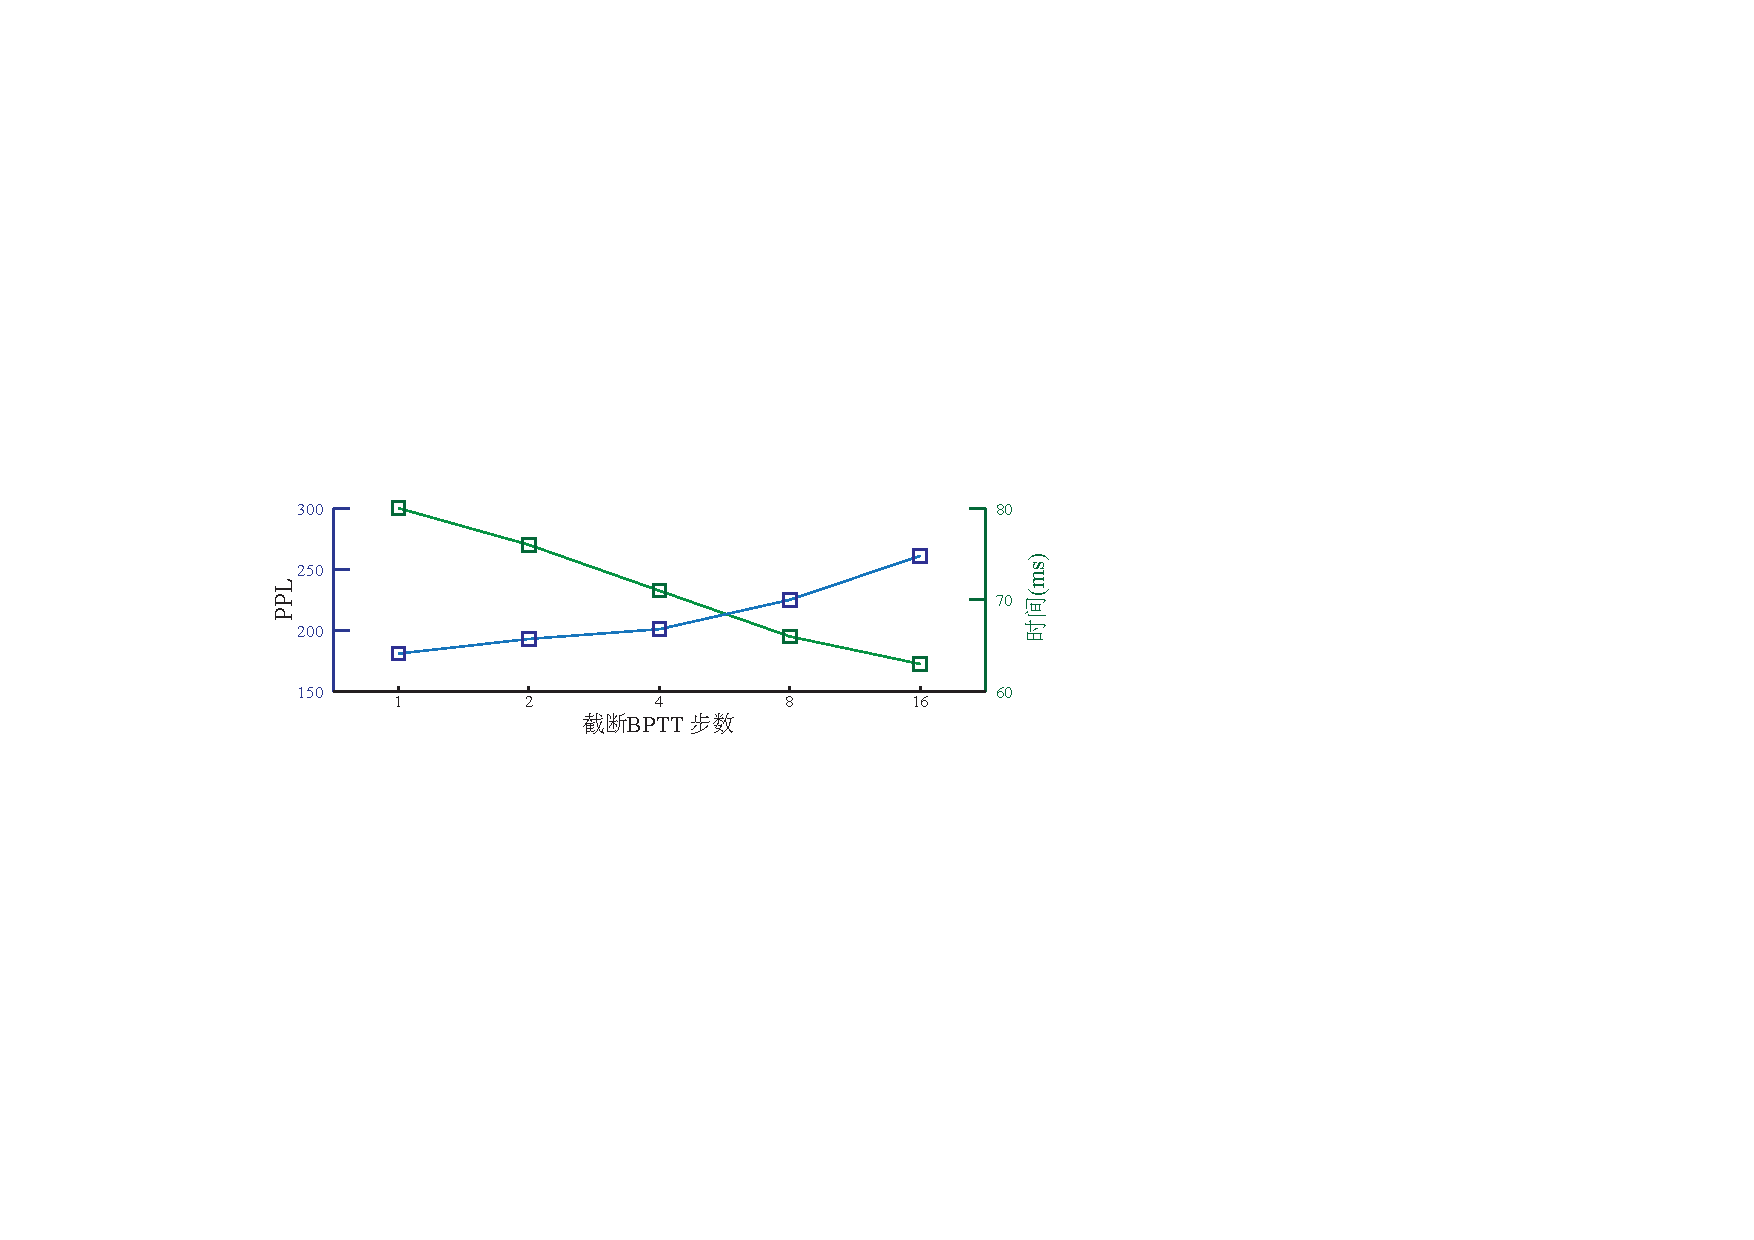
\includegraphics[width=0.65\columnwidth]{./figures/tbptt.pdf}
  \caption{Perplexity comparison of different Truncated BPTT Steps with the NCE and Blackout methods on Wikitext-2 dataset.}\label{fig:tbptt}
\end{figure}


\subsection{All Experiments Benchmark}

\begin{table}[t]
%\setlength{\abovecaptionskip}{0pt}
%\setlength{\abovedisplayskip}{0pt}
  \centering
  \caption{Perplexity and Word Error Rate on Wikitext-2,  WikiText-103 and One Billion Word Datasets.\label{tab:summary_ppl}}
\begin{tabular}{llcc}
  \toprule
数据集& 算法& 验证集(PPL/ WER) & 测试集(PPL/WER) \\ \midrule
 \multirow{2}{*}{WikiText-2}&GRU + Softmax&172.64 / 77.49\%&162.09 / 77.07\% \\
  &GRU + NCE~\upcite{DBLP:journals/jmlr/GutmannH10}&217.84 / 78.26\%&199.54 / 78.02\%\\
  &GRU + Blackout~\upcite{DBLP:journals/iclr/JiVSAD15}&221.15 / 77.72\%&199.56 / 77.50\% \\
  &GRU + cHSM + unigram~\upcite{DBLP:conf/acl/ChenGA16}&253.18 / 78.25\%&236.61 / 78.02\%\\
  &GRU + p-tHSM + unigram~\upcite{DBLP:conf/nips/MikolovSCCD13}&218.42 / 78.15\%&216.05 / 78.15\%\\
  &GRU + p-tHSM + bigram~\upcite{DBLP:journals/coling/BrownPdLM92}&186.23 / 78.15\%&189.58 / 78.15\%\\\midrule
   \multirow{2}{*}{WikiText-103} &GRU + Softmax&130.38 / 72.15\%&136.83 / 72.37\%\\
 &GRU + NCE~\upcite{DBLP:journals/jmlr/GutmannH10}&164.78 / 73.22\%&165.01 / 73.34\%\\
  &GRU + Blackout~\upcite{DBLP:journals/iclr/JiVSAD15}&163.99 / 73.18\%&162.76 / 74.22\%\\
  &GRU + cHSM + unigram~\upcite{DBLP:conf/acl/ChenGA16}&171.81 / 73.42\%&166.74 / 73.18\%\\
  &GRU + p-tHSM + unigram~\upcite{DBLP:conf/nips/MikolovSCCD13}&165.70 / 73.53\%&166.11 / 72.44\%\\
  &GRU + p-tHSM + bigram~\upcite{DBLP:journals/coling/BrownPdLM92}&164.15 / 78.15\%&163.55 / 77.85\%\\\midrule
  \multirow{2}{*}{One Billion Word} &GRU + Softmax&330.38 / 88.15\%&330.83 / 88.37\%\\
 & GRU + NCE~\upcite{DBLP:journals/jmlr/GutmannH10}&272.07 / 84.83\%&276.11 / 84.34\%\\
  &GRU + Blackout~\upcite{DBLP:journals/iclr/JiVSAD15}&268.67 / 84.23\%&266.11 / 84.18\%\\
 & GRU + cHSM + unigram~\upcite{DBLP:conf/acl/ChenGA16}&225.36 / 80.32\%&224.11 / 79.42\%\\
 & GRU + p-tHSM + unigram~\upcite{DBLP:conf/nips/MikolovSCCD13}&231.44 / 87.53\%&236.11 / 82.53\%\\
  &GRU + p-tHSM + bigram~\upcite{DBLP:journals/coling/BrownPdLM92}& 221.55 / 81.15\%&218.70 / 83.15\%\\
  \bottomrule
\end{tabular}
\end{table}